\section{Marco de Trabajo SCRUM}\label{Scrum}

Para la creación de la aplicación Web3 se ha seguido un marco de trabajo
inspirado en \textbf{SCRUM} para un desarrollo ágil. Este marco de trabajo está
fundamentado por la existencia de etapas de tiempo previamente establecidas
donde se enfoca la carga de trabajo, consiguiendo un producto mínimamente
viable en cada una de ellas. Estas etapas de tiempo se conocen por el nombre de
Sprints, y cada uno de ellos se divide en diferentes fases: planificación del
Sprint, realización del Sprint, con reuniones diarias, y retrospectiva del
Sprint. En la Figura \ref*{fig:scrum-imagen} se muestra el flujo de trabajo que
se suele seguir en la metodología SCRUM.

\begin{figure}[htb!]
    \centering
    \caption{Metodología SCRUM} \label{fig:scrum-imagen}
    \centering
    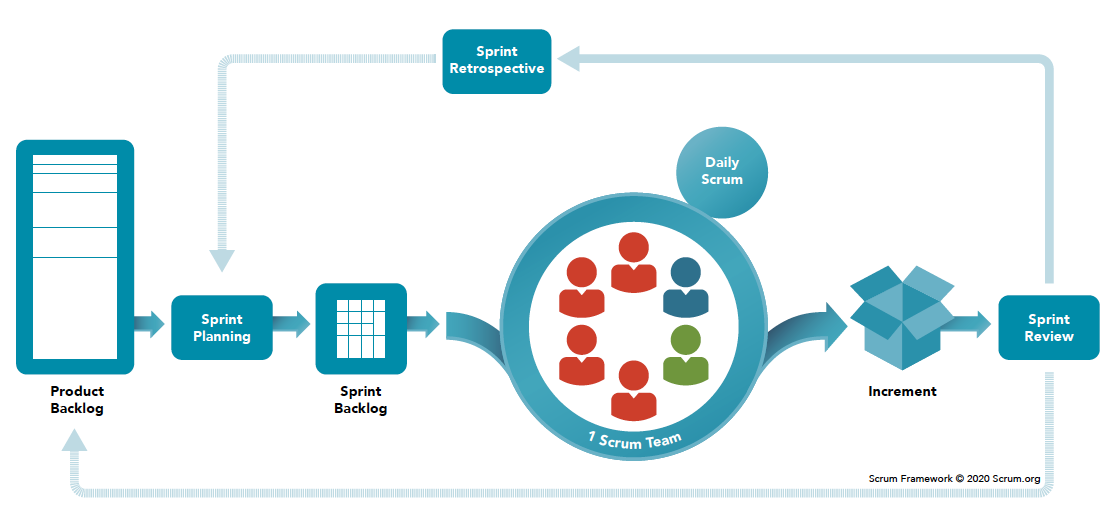
\includegraphics[scale=0.4]{./Ilustraciones/scrum.png}\\
    \textbf{Fuente:} www.scrum.org [\url{https://www.scrum.org/learning-series/what-is-scrum}]
\end{figure}

\textbf{Planificación del Sprint}: En esta fase, se definen
los objetivos del sprint, identifican las tareas necesarias para cumplir esos
objetivos y determinan la cantidad de trabajo que se puede realizar en el
sprint.

\textbf{Sprint}: Esta es la fase en la que se realiza el trabajo. Durante el sprint, se
trabaja en las tareas definidas en la planificación del sprint
para lograr los objetivos establecidos.

\textbf{Reunión diaria}: En esta fase, el equipo Scrum se reúne diariamente para revisar
el progreso del trabajo, identificar cualquier problema y hacer ajustes
necesarios para alcanzar los objetivos del sprint.

\textbf{Revisión del Sprint}: Al final del sprint, el equipo Scrum se reúne para revisar
el trabajo completado y demostrar los resultados a los interesados. Esto ayuda
a identificar los logros y también a las áreas donde se pueden mejorar.

\textbf{Retrospectiva del Sprint}: En esta fase, el equipo Scrum reflexiona sobre el
sprint anterior y discute qué se hizo bien y qué se puede mejorar en el próximo
sprint.

\textbf{Planificación de lanzamiento}: Si se han completado múltiples sprints, el equipo
Scrum se reúne para planificar la entrega del producto final al cliente.

A la hora de hacerlo, al no tener un "equipo", sino ser únicamente una persona,
la \textbf{planificación} del sprint se realizaba mediante el uso de
Trello[\ref{Trello}], añadiendo tareas, y colocando sus respectivos "tests",
que en su mayoría son validaciones por parte de personas externas.

La \textbf{realización del sprint} se realizaba en diferentes apartados, los
cuales son: \\

La parte de \textbf{diseño} realizado en Figma[Sección \ref{Figma}]
\begin{itemize}
    \item Diseño de componentes
    \item Diseño de páginas con los componentes diseñados
\end{itemize}

La parte de \textbf{desarrollo} realizado en Figma[Sección \ref{VSCode}]
haciendo uso de las distintas herramientas antes mencionadas[Capítulo
        \ref{recursos}].
\begin{itemize}
    \item Desarrollo de la página para poder colocar los componentes
    \item Desarrollo de los componentes e insertarlos de forma adecuada en la página
\end{itemize}

La parte de \textbf{validación} realizado con Lighthouse[Sección
        \ref{lighthouse}] y SonarQube[Sección \ref{sonarqube}]
\begin{itemize}
    \item Siguiendo el consejo antes mencionado de SonarQube, se pasaba el test antes de
          hacer un \textit{push}, comprobando la posible existencia de Code Smells, bugs,
          vulnerabilidades, etc.
    \item A la hora de pasar la validación de Lighthouse se hizo cada vez que se hacía un
          \textit{merge} a la rama principal, se pasaba este test para ver las posibles
          fallas de accesibilidad que tenía la página en ese momento y poder
          solucionarlas.\end{itemize}